% ====================================================================
% graphite_ica_ch2_v4-06.tex — Chapter 2 (v4: 코인 하프셀 엔트로피·가역 발열
%                               통계열역학 챕터)
%   출발 skeleton: graphite_ica_ch2_v3.tex (Bernardi 가역열 survey, 얇은 출발)
%   v4 재편(고유 챕터): 점유 분포를 명시 전개해 가역 발열을 통계열역학으로 닫는다 —
%     분배함수 Z → 점유 분포 ⟨n⟩(=Ch1 logistic 기원) → configurational/vibrational/
%     electronic 엔트로피(세 분포: 격자기체·포논 BE·전자 FD) → 봉우리 겹침 가중·
%     상호작용 w_eff(Ω)·히스테리시스 분기 → 극한 코너 → 가역 발열 합성.
%   범위: 코인 하프셀(단일 전극 vs Li) ∂U/∂T·가역열. 전셀 합성은 범위 외.
%   Ch1(graphite_ica_ch1 v8-11): forward dQ/dV. 재유도 X — 결과 인용
%     (logistic·U_j·ΔS_rxn·w=RT/F).
%   상태: v4 챕터판. 실데이터 round-trip 실증·v9 통합은 교수님 검토 후.
%   build: xelatex 2-pass (kotex + TikZ).
% ====================================================================
\documentclass[11pt,a4paper]{article}
\usepackage[margin=22mm]{geometry}
\usepackage{kotex}
\setmonofont{D2Coding}[Scale=MatchLowercase]
\usepackage{amsmath,amssymb,mathtools,bm}
\usepackage{booktabs,longtable,array}
\usepackage{enumitem}
\usepackage{amsthm}
\usepackage{tikz}
\usetikzlibrary{arrows.meta,calc,decorations.pathreplacing,positioning}
\usepackage{hyperref}
\usepackage{fancyhdr}
\usepackage{lastpage}
\usepackage{setspace}
\setstretch{1.12}
\setlength{\parskip}{0.45em}\setlength{\parindent}{0pt}\setlength{\headheight}{14pt}
\setlength{\emergencystretch}{2em}
\hypersetup{colorlinks=true, linkcolor=blue, urlcolor=blue, citecolor=blue,
  pdftitle={코인 하프셀 엔트로피·가역 발열의 통계열역학 — Chapter 2 (v4)}}
\pagestyle{fancy}\fancyhf{}
\lhead{흑연 음극 $dQ/dV$ — Ch.2 (v4, 엔트로피의 통계열역학)}\rhead{\thepage/\pageref{LastPage}}
\renewcommand{\headrulewidth}{0.4pt}
\newtheorem*{keybox}{핵심}
\newtheorem*{srcbox}{문헌 근거}
\newtheorem*{warnbox}{주의}
\newtheorem*{distbox}{분포 관점}
\newcommand{\dd}{\mathrm{d}}
\newcommand{\rxn}{\mathrm{rxn}}
\newcommand{\eq}{\mathrm{eq}}
\newcommand{\rev}{\mathrm{rev}}
\newcommand{\irr}{\mathrm{irr}}
\newcommand{\oc}{\mathrm{oc}}
\newcommand{\config}{\mathrm{config}}
\newcommand{\vibr}{\mathrm{vib}}
\newcommand{\elec}{\mathrm{el}}
\newcommand{\eff}{\mathrm{eff}}
\newcommand{\kB}{k_{\mathrm{B}}}
\newcommand{\avg}[1]{\langle #1\rangle}
\renewcommand{\theequation}{2.\arabic{equation}}
\renewcommand{\thesection}{2.\arabic{section}}
\title{\textbf{\LARGE Chapter 2}\\[0.35em]\Large 코인 하프셀 엔트로피와 가역 발열의 통계열역학\\[0.2em]\large — 점유 분포에서 $\partial U/\partial T\cdot\Delta S(x)\cdot\dot Q_\rev$ 로 (v4)}
\author{}\date{}

\begin{document}
\maketitle

% ====================================================================
\section*{서 — 왜 엔트로피에는 통계가 필요한가}
\addcontentsline{toc}{section}{서}
% ====================================================================
Chapter 1 은 흑연 음극의 $\dd Q/\dd V$ 한 곡선을, 전이별 평형 중심 전위
$U_j(T)=(-\Delta H_{\rxn,j}+T\,\Delta S_{\rxn,j})/F$ 위에 세운 평형 종과, 그 위에 얹힌 동역학 꼬리로
설명했다. 그 한 곡선의 모양은 결국 한 가지 미시적 사실에서 나온다: \emph{리튬 이온이 흑연의 가용
자리들에 어떻게 분포하는가}. 평형 전위는 그 분포가 한 자리를 더 채울 때 드는 전기화학적 대가이고,
$\dd Q/\dd V$ 봉우리는 분포가 가장 잘 받아들이는 전위 구간이다. Chapter 1 은 그 분포의 \emph{평형
모양}(logistic 종)을 forward 방향으로 세웠다.

이 장은 같은 분포를 \emph{다른 렌즈}로 다시 본다 — 온도의 렌즈다. 분포에는 폭이 있고, 폭에는
\emph{흩어짐}이 있으며, 흩어짐의 척도가 곧 엔트로피다. 그러므로 평형 전위의 온도 의존
$\partial U/\partial T$ 는 ``Chapter 1 에 우연히 딸려 온 부산물''이 아니라, \emph{같은 점유 분포가
가진 엔트로피를 온도가 드러낸 것}이다. 전지가 충방전하며 흡수$\cdot$방출하는 \emph{가역(엔트로피)
발열}은 바로 이 분포를 한 충전 상태(SOC)에서 다른 SOC 로 \emph{재배열하는 열}이다 \cite{huggins2009}.

여기서 통계가 불가피해진다. 엔트로피는 한 미시상태의 성질이 아니라 \emph{미시상태들의 분포}의 성질이다.
따라서 측정된 엔트로피 계수 $\partial U/\partial T(x)$ 를 ``이해''하려면 — 한 곡선의 기울기로 외우는 데
그치지 않으려면 — Li(와 그에 동반하는 전자, 격자 진동)의 점유 \emph{분포}를 명시적으로 세우고, 그
분포의 엔트로피를 직접 계산해야 한다. 이 장의 골격은 그 한 줄이다:
\[
\boxed{\;\text{점유 분포}\;\to\;S_\config,\,S_\vibr,\,S_\elec\;\to\;\frac{\partial U}{\partial T}(x)=\frac{\Delta S(x)}{F}\;\to\;\dot Q_\rev=-I\,T\,\frac{\partial U}{\partial T}\;}
\]
곧 분배함수에서 출발해 점유 분포를 얻고(\S\ref{sec:partition}), 그 분포의 흩어짐에서
configurational 엔트로피를 끌어내고(\S\ref{sec:config}), 격자 진동과 전도 전자의 분포가 주는 두
엔트로피를 더해(\S\ref{sec:vibel}) 총 엔트로피 계수를 세운 뒤(\S\ref{sec:total}), 그것이 Bernardi
에너지 수지의 가역열에 어떻게 들어가는지(\S\ref{sec:bernardi}) 본다. 그 위에서 실제 흑연 곡선이
요구하는 세 가지 추가 — 봉우리 겹침(\S\ref{sec:overlap}), 상호작용과 히스테리시스
(\S\ref{sec:omega}), 극한 코너(\S\ref{sec:limits}) — 를 닫고, 가역 발열 프로파일로 합성한다
(\S\ref{sec:synth}).

\begin{keybox}
\textbf{Chapter 1 과 Chapter 2 의 분업.} Chapter 1 = 점유 분포의 \emph{평형 모양}(forward
$\dd Q/\dd V$). Chapter 2 = 그 \emph{같은 분포}의 엔트로피$\cdot$온도 의존$\cdot$가역 발열. 본 장은 Ch1
을 재유도하지 않는다 — logistic 점유 $\xi_\eq$, 전이 중심 $U_j$, 반응 엔트로피 $\Delta S_{\rxn,j}$,
폭 $w=RT/F$ 를 \emph{결과로 인용}하고, 그것들이 실은 격자기체 분포의 통계적 산물임을 보인다. 범위는
\emph{코인 하프셀}(흑연 전극 vs.\ Li 금속)의 단일 전극 엔트로피 계수다. 전셀 합성
($\partial U_\mathrm{cell}=\partial U_\mathrm{cat}-\partial U_\mathrm{an}$)은 본 장의 범위 밖이다.
\end{keybox}

% ====================================================================
\section{격자기체 분배함수에서 점유 분포로 — Chapter 1 logistic 의 기원}\label{sec:partition}
% ====================================================================
출발점은 가장 단순한 통계 단위다: 흑연 격자의 \emph{자리(site)} 하나가 Li 로 채워지거나 비거나
하는 두 상태. 이 한 자리의 분포를 세우는 데서 Chapter 1 의 모든 평형 구조 — logistic 점유, 전이 폭
$w$, 봉우리 모양 — 가 통계적으로 따라 나온다.

\subsection{단일 자리 대정준 분배함수}
한 자리는 외부 저장조(전해질 속 Li$^+$ + 외부 회로 전자)와 입자를 주고받으므로, 자연스러운 앙상블은
\emph{대정준(grand canonical)}이다. 자리가 비면 에너지 $0\cdot$점유수 $0$, Li 가 점유하면 자리
에너지 $\varepsilon_0$$\cdot$점유수 $1$ 이고, 저장조의 전기화학 퍼텐셜이 $\mu$ 이다. 두 상태에 대한
대분배함수는
\begin{equation}
Z_1 \;=\; \sum_{n=0,1} e^{-\beta(\varepsilon_0 - \mu)\,n}
       \;=\; 1 + e^{-\beta(\varepsilon_0-\mu)},
\qquad \beta\equiv\frac{1}{\kB T},
\label{eq:Z1}
\end{equation}
이다 \cite{hill}. 자리의 평균 점유는 $\avg{n}=\beta^{-1}\,\partial\ln Z_1/\partial\mu$ 로, 곧
\begin{equation}
\boxed{\;\avg{n}
   \;=\;\frac{e^{-\beta(\varepsilon_0-\mu)}}{1+e^{-\beta(\varepsilon_0-\mu)}}
   \;=\;\frac{1}{1+e^{\,\beta(\varepsilon_0-\mu)}}\;}
\label{eq:occ}
\end{equation}
이다. 이것이 본 장의 첫 번째 \emph{분포}다 — 자리당 Li 점유 확률. 식~\eqref{eq:occ} 는
\emph{Fermi--Dirac 함수와 구조가 동형}이다(자리당 2-상태, Pauli 식 배타: 한 자리에 Li 0 또는 1).
이는 우연이 아니라, ``채워지거나 비거나''라는 같은 2-상태 통계에서 나온 같은 함수꼴이다.

\subsection{Chapter 1 의 logistic 은 이 분포다}
전기화학 퍼텐셜을 전극 전위에 묶으면 식~\eqref{eq:occ} 가 곧바로 Chapter 1 의 logistic 이 된다.
전이 $j$ 의 자리에 Li 를 넣는 전기화학 퍼텐셜은 전극 전위 $V$ 에 선형으로 $\mu=\mu_j^0-\sigma_d F\,(V-U_j)$
로 묶인다($\sigma_d=\pm1$ 충방전 부호, $U_j$ = 전이 중심, 그 정의가 $\mu(V{=}U_j)=\mu_j^0=\varepsilon_0$
이 되도록 잡힘 — 즉 중심에서 점유 $\tfrac12$). 이를 식~\eqref{eq:occ} 의 지수에 대입하면
$\varepsilon_0-\mu=\varepsilon_0-\mu_j^0+\sigma_d F(V-U_j)=\sigma_d F(V-U_j)$ 이고, 1몰당으로 환산
($N_A\kB=R$, $N_A e=F$)하면 $\beta(\varepsilon_0-\mu)=\sigma_d F(V-U_j)/(RT)=\sigma_d(V-U_j)/w$ 이
되어
\begin{equation}
\avg{n}\;=\;\xi_{\eq,j}(V,T)\;=\;\frac{1}{1+\exp\!\big[\,\sigma_d\,(V-U_j)/w\big]},
\qquad
\boxed{\;w=\frac{RT}{F}\;}
\label{eq:logistic}
\end{equation}
가 된다 — 이것이 Chapter 1 이 forward 로 세운 평형 점유 logistic 이다(방전 $\sigma_d{=}+1$ 에서
$V\!<\!U_j$ 일 때 $\avg{n}\to1$, 곧 낮은 전위에서 Li 가 채워짐). \textbf{여기서 본 장의 첫
번째 봉합이 일어난다}: Chapter 1 의 평형 점유 $\xi_\eq$ 는 \emph{격자기체 자리의 점유 확률 분포}이고,
그 폭을 정하는 $w=RT/F$ 는 \emph{분포의 너비}(열적 흩어짐)다. $RT/F$ 가 온도에 비례한다는 사실 자체가
이미 ``이 폭은 엔트로피적 흩어짐''임을 말한다 — \S\ref{sec:config} 에서 이 폭이 곧 configurational
엔트로피의 부분몰임을 정량으로 확인한다.

\begin{distbox}
$\dd Q/\dd V$ 봉우리 모양 $g_j\equiv\partial\xi_j/\partial V = \xi_j(1-\xi_j)/w$ 는 점유 분포
\eqref{eq:logistic} 의 \emph{도함수}, 곧 로지스틱 분포의 밀도다. 봉우리의 높이$\cdot$폭은 분포의
열적 흩어짐 $w=RT/F$ 가 정한다. Chapter 1 의 ``봉우리''는 통계적으로 \emph{점유 분포의 미분}이다.
\end{distbox}

\subsection{다자리 평균장 — Bragg--Williams 격자기체}
단일 자리 \eqref{eq:occ} 는 자리들이 서로 무관할 때의 한계다. 실제 흑연 stage 는 점유한 Li 끼리
상호작용(반발$\cdot$인력)하므로, $N$ 자리 격자기체를 평균장(Bragg--Williams)으로 닫는다. 채움률
$\theta\equiv\avg{n}$ 의 한 자리당 깁스 에너지는
\begin{equation}
g(\theta)\;=\;g_0 \;+\; RT\big[\theta\ln\theta+(1-\theta)\ln(1-\theta)\big]
          \;+\; \Omega\,\theta(1-\theta),
\label{eq:bw}
\end{equation}
이다. 둘째 항은 점유의 \emph{섞임}(configurational) 항(곧 \S\ref{sec:config} 의 엔트로피),
셋째 항은 평균장 상호작용($\Omega>0$ 반발 = 상분리 경향, $\Omega<0$ 인력 = 정렬 경향)이다.
평형 조건 $\mu=\partial g/\partial\theta$ 에서
\begin{equation}
\mu(\theta)-\mu_0
   \;=\; RT\,\ln\frac{\theta}{1-\theta} \;+\; \Omega\,(1-2\theta),
\label{eq:mu_bw}
\end{equation}
가 나오고 \cite{bazant2013}, $\Omega=0$ 이면 \eqref{eq:logistic} 의 logistic 으로 정확히 환원된다(상호작용 없는
이상 격자기체 = Chapter 1 의 기본 logistic). $\Omega$ 가 분포를 비트는 양상 — 봉우리를 좁히고,
$\Omega>2RT$ 에서 분포를 둘로 쪼개(bimodal = 상분리) plateau 를 만드는 — 은 \S\ref{sec:omega} 에서
다룬다. 곧 \textbf{흑연의 stage plateau 자체가 점유 분포의 상호작용에 의한 변형}이다.

% ====================================================================
\section{분포에서 configurational 엔트로피로}\label{sec:config}
% ====================================================================
이제 \S\ref{sec:partition} 의 점유 분포에서 엔트로피를 \emph{직접} 끌어낸다. 이 절이 본 장의 심장이다 —
측정된 $\partial U/\partial T(x)$ 의 ``봉우리 내부'' $x$-의존이 어디서 오는지를 분포 한 줄로 닫는다.

\subsection{점유 분포의 Boltzmann/Shannon 엔트로피}
한 자리가 점유 확률 $\theta$, 공석 확률 $1-\theta$ 인 2-상태 분포를 가질 때, 그 분포의 엔트로피는
Boltzmann--Gibbs/Shannon 정의 $S=-R\sum_i p_i\ln p_i$ 에서 곧바로
\begin{equation}
\boxed{\;S_\config(\theta)\;=\;-R\big[\theta\ln\theta+(1-\theta)\ln(1-\theta)\big]\;}
\qquad(\text{자리 1몰당})
\label{eq:Sconfig}
\end{equation}
이다. 이것이 식~\eqref{eq:bw} 의 $RT[\theta\ln\theta+(1-\theta)\ln(1-\theta)]$ 항을 엔트로피로
다시 읽은 것이다($-TS_\config$). 통계적 의미는 직접적이다: $\theta=\tfrac12$ 에서 자리들이 점유/공석을
가장 ``모르는'' 상태 = 최대 흩어짐 = $S_\config$ 최대($R\ln2$); $\theta\to0$ 또는 $\theta\to1$ 에서
배열이 단 하나로 확정되어 $S_\config\to0$. 곧 \textbf{엔트로피는 점유 분포가 얼마나 퍼져 있는지를
재는 양}이며, 이것이 ``엔트로피에 통계가 필요한 이유''의 구체다.

\subsection{부분몰 엔트로피 — $\partial U/\partial T$ 의 봉우리 내부 항}
가역 발열에 들어가는 것은 \emph{Li 1몰을 더 삽입할 때}의 엔트로피 변화, 곧 부분몰 엔트로피다.
식~\eqref{eq:Sconfig} 를 $\theta$ 로 미분하면
\begin{equation}
\boxed{\;\frac{\partial S_\config}{\partial\theta}\;=\;-R\,\ln\frac{\theta}{1-\theta}\;}
\label{eq:partial_Sconfig}
\end{equation}
이다. 이 한 항이 측정 엔트로피 계수의 \emph{$x$-의존(봉우리 내부)} 부분이다. 부호와 발산이 물리를
그대로 말한다: 희박($\theta\to0$, Li 거의 없음)에서 한 개를 더 넣을 자리가 무수히 많아 부분몰
엔트로피가 $+\infty$ 로 발산; 만충($\theta\to1$)에서는 남은 자리가 거의 없어 $-\infty$ 로 발산.
중간 $\theta=\tfrac12$ 에서 $0$ — 분포가 가장 퍼진 곳에서 한 개 더 넣어도 흩어짐이 변하지 않는다.

\begin{figure}[t]
\centering
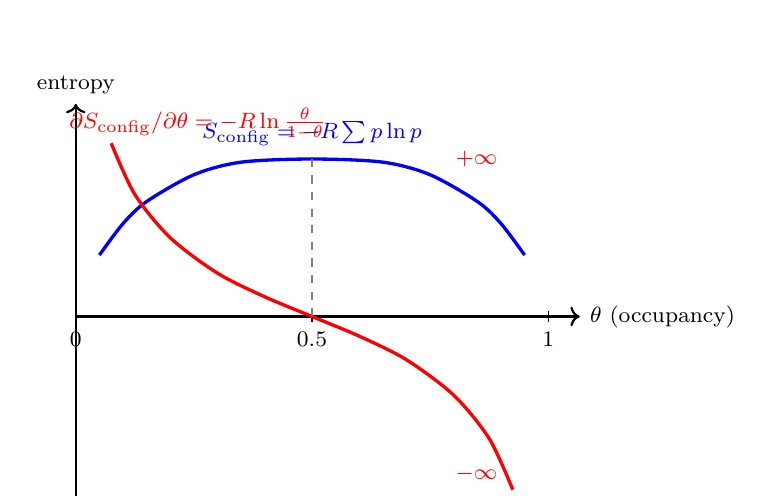
\begin{tikzpicture}[x=1.0cm,y=1.0cm]
  % axes
  \draw[->,thick] (0,0) -- (6.4,0) node[right]{\footnotesize $\theta$ (occupancy)};
  \draw[->,thick] (0,-2.4) -- (0,2.7) node[above]{\footnotesize entropy};
  \foreach \t/\lab in {0/0,3/0.5,6/1}{\draw (\t,0.07)--(\t,-0.07) node[below]{\footnotesize \lab};}
  % S_config dome:  S = -R[th ln th + (1-th)ln(1-th)], scaled, peak R ln2 at th=0.5
  % sample points (theta, S/R) scaled y = 2.0*S/Rln2
  \draw[blue,very thick,smooth]
    plot coordinates {(0.30,0.78)(0.60,1.18)(0.90,1.46)(1.50,1.80)(2.10,1.96)(3.00,2.00)
                      (3.90,1.96)(4.50,1.80)(5.10,1.46)(5.40,1.18)(5.70,0.78)};
  \node[blue] at (3.0,2.32) {\footnotesize $S_\mathrm{config}=-R\sum p\ln p$};
  % partial molar dS/dtheta = -R ln(theta/(1-theta)): + at small theta, - at large
  \draw[red,very thick,smooth]
    plot coordinates {(0.45,2.2)(0.75,1.55)(1.20,1.0)(1.80,0.55)(2.40,0.25)(3.00,0.0)
                      (3.60,-0.25)(4.20,-0.55)(4.80,-1.0)(5.25,-1.55)(5.55,-2.2)};
  \node[red] at (1.55,2.45) {\footnotesize $\partial S_\mathrm{config}/\partial\theta=-R\ln\frac{\theta}{1-\theta}$};
  \draw[dashed,gray] (3,0)--(3,2.0);
  \node[red,anchor=west] at (4.7,2.0) {\footnotesize $+\infty$};
  \node[red,anchor=west] at (4.7,-2.0) {\footnotesize $-\infty$};
\end{tikzpicture}
\caption{The occupation distribution and its entropy. Blue: configurational entropy
$S_\mathrm{config}(\theta)$, a dome peaking at $R\ln2$ where the distribution is most spread
($\theta=\tfrac12$). Red: the partial-molar entropy $\partial S_\mathrm{config}/\partial\theta
=-R\ln[\theta/(1-\theta)]$, the in-peak $x$-dependence of $\partial U/\partial T$ — diverging
$+\infty$ in the dilute limit ($\theta\to0$) and $-\infty$ at full filling ($\theta\to1$),
crossing zero at the center. The width $w=RT/F$ of Chapter~1's logistic already carries this term.}
\label{fig:occ_entropy}
\end{figure}

\subsection{Chapter 1 의 $w=RT/F$ 가 이미 이 항을 담고 있다}\label{sub:w_carries}
이제 두 번째 봉합이다. 식~\eqref{eq:logistic} 의 점유 logistic 을 전위에 대해 역함수로 풀면
$V=U_j+w\ln[(1-\xi_\eq)/\xi_\eq]$ 이다($\xi_\eq=\avg{n}$ = 채움률). 이를 \emph{탈리튬화 진행률}
$\xi\equiv1-\xi_\eq$(\S\ref{sub:sign} 부호 규약, $\ln[(1-\xi_\eq)/\xi_\eq]=\ln[\xi/(1-\xi)]$)로 바꿔 쓰면
\begin{equation}
V(\xi)\;=\;U_j\;+\;\frac{RT}{F}\,\ln\frac{\xi}{1-\xi}
\label{eq:Vxi}
\end{equation}
이고($\xi$ = 전이 $j$ 의 국소 탈리튬화 진행률), 이를 온도로 미분하면
\begin{equation}
\boxed{\;\frac{\partial V}{\partial T}\Big|_\xi
   \;=\;\underbrace{\frac{\Delta S_{\rxn,j}}{F}}_{\text{표준(중심)}}
   \;+\;\underbrace{\frac{R}{F}\,\ln\frac{\xi}{1-\xi}}_{\text{config 분포}}\;}
\label{eq:dVdT}
\end{equation}
가 나온다. 둘째 항은 정확히 식~\eqref{eq:partial_Sconfig} 의 부분몰 configurational 엔트로피를 $F$ 로
나눈 것이다($\partial S_\config/\partial\theta = -R\ln[\theta/(1-\theta)] = +R\ln[\xi/(1-\xi)]$,
$\xi=1-\theta$ 규약). 곧 \textbf{Chapter 1 이 logistic 의 폭으로 $RT/F$ 를 쓴 그 순간, 봉우리 내부
configurational 부분몰 엔트로피는 이미 모델 안에 들어 있었다} — 별도로 더할 필요가 없다. 첫째 항
$\Delta S_{\rxn,j}/F$ 는 전이 $j$ 의 \emph{중심 표준값}($\xi=\tfrac12$, config$=0$)이고, 둘째 항이
중심에서 벗어난 $x$ 에서의 분포 보정이다.

\begin{warnbox}
\textbf{이중계산 B 금지.} 식~\eqref{eq:dVdT} 의 $\Delta S_{\rxn,j}$ 는 반드시 \emph{전이 중심
($\xi=\tfrac12$)의 표준값}으로 둔다. 봉우리 내부의 $x$-의존은 둘째 항(폭 $w=RT/F$ 가 주는 분포 항)이
\emph{이미} 담고 있으므로, configurational 기여를 $\Delta S_{\rxn,j}$ 안에 또 한 번 넣으면 같은 물리를
두 번 세는 것이다. 측정 $\Delta S(x)$ = (중심 표준 $\Delta S_{\rxn,j}$) $+$ (분포 config $R\ln[\xi/(1-\xi)]$)
$+$ (vib$\cdot$electronic — 이들은 중심값에 흡수, \S\ref{sec:vibel}). 세 출처는 \emph{별개 항}이고,
어느 하나를 다른 하나에 겹쳐 넣지 않는다.
\end{warnbox}

\subsection{부호 규약}\label{sub:sign}
본 장은 Chapter 1 과 동일한 부호 규약을 쓴다. $\xi$ = 전이의 \emph{탈리튬화 진행률}(Li 가 빠져나가는
방향으로 $\xi:0\to1$), 채움률 $\theta=1-\xi$. 따라서 식~\eqref{eq:partial_Sconfig} 의 채움 기준
$-R\ln[\theta/(1-\theta)]$ 는 진행률 기준으로 $+R\ln[\xi/(1-\xi)]$ 가 되어 식~\eqref{eq:dVdT} 의
둘째 항과 일치한다. 발산 방향: 희박 Li($\xi\to1$, 거의 다 빠짐)에서 config 부분몰 $+\infty$ —
이것이 저-$x$ 큰 양의 $\Delta S$($+29$ J\,mol$^{-1}$K$^{-1}$, \S\ref{sec:synth})의 주원천이다;
만충($\xi\to0$)에서 $-\infty$. 엔트로피 계수와 반응 엔트로피는 $\partial U/\partial T=\Delta S/F$ 로
묶이며($n=1$, Li 1몰당, \S\ref{sec:bernardi}), 전자 삽입항 $\Delta S_e<0$ 규약은 Chapter 1 v9 와
일관된다(\S\ref{sec:vibel}).

이로써 측정 $\partial U/\partial T(x)$ 비선형의 한 \emph{출처}가 분포에서 자동 생성됨을 보았다:
전이 폭 안에서 $\xi$ 가 $0\!\to\!1$ 로 움직이면 둘째 항이 $-\infty\!\to\!+\infty$ 로 쓸려, 측정
계수를 봉우리마다 휘게 한다. 나머지 출처(봉우리 겹침)는 \S\ref{sec:overlap} 에서 닫는다.

% ====================================================================
\section{나머지 두 분포 — 격자 진동(포논)과 전도 전자}\label{sec:vibel}
% ====================================================================
configurational 엔트로피는 ``어느 자리에 Li 가 있는가''의 흩어짐이었다. 그러나 Li 가 삽입되면 \emph{격자
자체}도 바뀐다 — 진동 모드가 부드러워지거나 굳고(포논 분포 변화), 호스트의 전자 구조가 바뀐다(전도 전자
분포 변화). 가역 발열의 측정 엔트로피 계수에는 이 두 분포의 기여도 더해진다. 두 항 모두 \emph{분포}에서
유도되므로 본 장의 일관된 렌즈 안에 있다.

\subsection{vibrational 엔트로피 — 포논 Bose--Einstein 분포}
격자 진동은 보존(포논)이므로 모드 $k$(각진동수 $\omega_k$)의 점유는 Bose--Einstein 분포
$n_k=1/(e^{\beta\hbar\omega_k}-1)$ 를 따른다. 이 분포의 엔트로피는
\begin{equation}
S_\vibr\;=\;R\sum_k\Big[(1+n_k)\ln(1+n_k)-n_k\ln n_k\Big],
\qquad n_k=\frac{1}{e^{\beta\hbar\omega_k}-1},
\label{eq:Svib}
\end{equation}
이다(조화 근사, 자리 1몰당). configurational 분포(2-상태 격자기체)와 달리 이것은 \emph{무한
준위} 보존 분포의 엔트로피이지만, 같은 $-R\sum p\ln p$ 정신의 직접 산물이다. Li 삽입이 모드를
부드럽게(낮은 $\omega$) 만들면 $n_k$ 가 커져 $S_\vibr$ 증가, 굳히면 감소한다. 흑연에서 삽입 시
부분몰 $\Delta S_\vibr=\partial S_\vibr/\partial x$ 는 \emph{고-$x$(만충)에서 음의 baseline} 을 만든다 —
Reynier 등이 ``second contribution''(고분율 $\Delta S<0$)으로 보고한 항이 이것이다 \cite{reynier2003}.

\subsection{electronic 엔트로피 — Fermi--Dirac 분포(Sommerfeld)}
전도 전자는 페르미온이므로 에너지 $E$ 준위의 점유는 Fermi--Dirac 분포
$f(E)=1/(e^{\beta(E-E_F)}+1)$ 를 따른다 — 이미 식~\eqref{eq:occ} 와 같은 함수꼴이다(자리당 2-상태와
준위당 2-상태가 같은 통계). 페르미 면 부근 $\sim\kB T$ 폭만 흩어지므로, 저온 전개(Sommerfeld)에서
전자 엔트로피는
\begin{equation}
\boxed{\;S_\elec\;=\;\frac{\pi^2}{3}\,\kB^2\,T\,g(E_F)\;}
\label{eq:Sel}
\end{equation}
로, $T$ 에 \emph{선형}이고 페르미 준위 상태밀도 $g(E_F)$ 에 비례한다 \cite{ashcroftmermin}. 삽입 시 부분몰
$\Delta S_e=\partial S_\elec/\partial x$ 는 호스트의 $g(E_F)$ 변화로 결정된다 — 본 장 부호 규약에서
삽입 기준 $\Delta S_e<0$(Chapter 1 v9 일관). 크기는 호스트 종류가 가른다:

\begin{itemize}[leftmargin=1.4em,itemsep=2pt]
\item \textbf{흑연 하프셀}: 흑연은 준금속이라 $g(E_F)$ 가 작아 $S_\elec$ 기여가 거의 무시할 만하다
($\Delta S_e\approx0$). 흑연의 측정 $\partial U/\partial T(x)$ 는 사실상 config $+$ vib 두 분포로 닫힌다.
\item \textbf{LCO(Li$_x$CoO$_2$) 하프셀}: 탈리튬화 과정에 절연체$\to$금속 전이(MIT)가 있어 한 전이
구간에서 $g(E_F)$ 가 급변한다. 그 구간에서만 $\Delta S_e$ 가 $x$-의존을 유지하며(\emph{게이트}처럼
켜진다), 본 장 분포 사슬에 FD 항으로 들어간다. 이것이 Chapter 1 v9 의 전자항 확장이 닿는 지점이다.
\end{itemize}

\begin{distbox}
\textbf{한 챕터, 세 분포.} 측정 엔트로피 계수에 들어가는 세 항은 모두 \emph{분포의 엔트로피}다 —
(i) Li 점유의 격자기체 분포(config, 2-상태), (ii) 격자 진동의 포논 BE 분포(vib), (iii) 전도 전자의
FD 분포(electronic). 셋은 같은 $-R\sum p\ln p$ 정신에서 나오되 서로 다른 자유도를 센다. 이 장의 통일성은
바로 여기 있다: \emph{가역 발열은 이 세 분포를 재배열하는 열의 합}이다.
\end{distbox}

% ====================================================================
\section{총 엔트로피 계수 — 세 분포의 합}\label{sec:total}
% ====================================================================
\S\ref{sec:config}--\S\ref{sec:vibel} 의 세 분포를 한 곳에 모은다. 한 전이 $j$ 가 진행 중인 SOC 에서,
측정 엔트로피 계수는
\begin{equation}
\boxed{\;
\frac{\partial U}{\partial T}(x)\;=\;\frac{\Delta S(x)}{F},
\qquad
\Delta S(x)\;=\;
\underbrace{\Delta S^0_j}_{\substack{\text{표준(중심)}\\ \text{vib+el 흡수}}}
\;+\;
\underbrace{R\,\ln\frac{\xi}{1-\xi}}_{\substack{\text{config 분포}\\ \text{(폭 }w=RT/F)}}
\;+\;
\underbrace{\Delta S_e^{\,\mathrm{gate}}(x)}_{\substack{\text{FD, MIT 게이트}\\ \text{(LCO 한정)}}}
\;}
\label{eq:master}
\end{equation}
이다($n=1$, Li 1몰당). 세 항의 출처와 역할을 분명히 한다:

\begin{itemize}[leftmargin=1.4em,itemsep=3pt]
\item $\Delta S^0_j$ — 전이 $j$ 의 \emph{중심 표준값}($\xi=\tfrac12$). 여기에 vibrational
부분몰($\Delta S_\vibr$, 고-$x$ 음의 baseline)과 전자 항의 \emph{중심값}이 흡수된다. ``전이당 하나의
상수''로 두는 것이 이 항의 정의다.
\item $R\ln[\xi/(1-\xi)]$ — configurational 분포가 주는 \emph{봉우리 내부} $x$-의존. 폭 $w=RT/F$ 가
이미 담고 있으므로(\S\ref{sub:w_carries}) 별도 입력이 아니다. 부호: $\xi\to1$(희박)에서 $+\infty$,
$\xi\to0$(만충)에서 $-\infty$. ★이중계산 B 금지($\Delta S^0_j$ 에 또 더하지 말 것).
\item $\Delta S_e^{\,\mathrm{gate}}(x)$ — 한 전이 폭 안에서 $g(E_F)$ 가 급변할 때(LCO MIT)만 켜지는
$x$-의존 전자 항. 흑연 하프셀에서는 $\approx0$ 이라 사라지고, 측정 계수는 앞 두 항으로 닫힌다.
\end{itemize}

부호 종합(흑연 하프셀): config 가 저-$x$(희박, $\xi\to1$)에서 $+$ 로 크게 발산 → 전극 측정 계수가
저-$x$ 에서 양($\Delta S\approx+29$ J\,mol$^{-1}$K$^{-1}$ ⟹ $\partial U/\partial T=\Delta S/F\approx
+0.3$ mV/K, \S\ref{sec:overlap} 표~\ref{tab:verify} 와 정합); vib baseline 이 고-$x$ 에서 $\Delta S^0_j$
를 음으로 끌어내림 → 고-$x$ 흡열 신호. (full-cell potentiometric 보고의 $+3\!\sim\!4$ mV/K는 셀 정의
기준이라 전극 단독값과 척도가 다름 — \S\ref{sec:synth}.) \S\ref{sec:overlap} 에서 여러 전이가 겹칠 때
이 식이 용량 가중 평균으로 어떻게 확장되는지 닫는다.

% ====================================================================
\section{가역 발열 — Bernardi 에너지 수지를 분포 관점으로}\label{sec:bernardi}
% ====================================================================
지금까지 세운 엔트로피 계수가 \emph{측정 가능한 열}이 되는 다리를 놓는다. 전지 셀의 발열은 가역
(reversible, 엔트로피) 성분과 비가역(irreversible) 성분으로 갈린다. Bernardi, Pawlikowski, Newman 의
일반 에너지 수지 \cite{bernardi1985} 에서, 부반응$\cdot$혼합$\cdot$상변화를 무시한 단일 활물질 한계의
발열률은
\begin{equation}
\dot Q \;=\; I\,(U_\oc-V) \;-\; I\,T\,\frac{\partial U_\oc}{\partial T},
\label{eq:bernardi}
\end{equation}
이다($I>0$ 방전, $V$ 단자 전압, $U_\oc$ 개방회로(평형) 전위). 우변 첫 항 $I(U_\oc-V)=I\,\eta\ge0$ 은
과전압 $\eta$ 의 소산 — \emph{비가역열} $\dot Q_\irr$(2법칙상 항상 발열). 둘째 항이 \emph{가역열}
\begin{equation}
\boxed{\;\dot Q_\rev \;=\; -\,I\,T\,\frac{\partial U_\oc}{\partial T}
       \;=\; -\,\frac{I\,T}{F}\,\Delta S(x)\;,}
\label{eq:qrev}
\end{equation}
이며, $\partial U_\oc/\partial T$(엔트로피 계수)의 부호에 따라 흡열($\dot Q_\rev<0$) 또는 발열($>0$)이
된다 — 비가역열과 달리 \emph{양방향}이다 \cite{bernardi1985,standardised2024}.

\begin{distbox}
\textbf{가역 발열 = 분포 재배열 열.} 식~\eqref{eq:qrev} 의 $\Delta S(x)$ 는 식~\eqref{eq:master} 의
세 분포 엔트로피의 합이다. 곧 $\dot Q_\rev$ 은 충전이 SOC 를 $x$ 에서 $x+\dd x$ 로 옮길 때 Li 점유
분포(+포논+전자 분포)를 \emph{재배열하는 데 드는/나오는 열}이다. 충방전이 분포를 같은 경로로 되돌리면
($I\to-I$) 부호만 바뀌어 \emph{가역}이다. 측정 $\partial U/\partial T(x)$ 의 비선형은 이 분포의
$x$-의존이 그대로 찍힌 것이다.
\end{distbox}

\subsection{Chapter 1 의 $U_j(T)$ 에서 전이별 엔트로피 계수}
열역학적으로 엔트로피 계수가 곧 반응 엔트로피임을 명시한다. Chapter 1 의 전이별 평형 중심은
$U_j(T)=(-\Delta H_{\rxn,j}+T\,\Delta S_{\rxn,j})/F$ 였다. 온도로 미분하면
\begin{equation}
\boxed{\;\frac{\partial U_j}{\partial T}\;=\;\frac{\Delta S_{\rxn,j}}{F}\;,}
\label{eq:coeff}
\end{equation}
곧 각 전이의 (중심) 엔트로피 계수가 그 전이의 반응 엔트로피다. 같은 결과를 통계열역학으로 보면:
$\Delta G=-nF U_\oc$ 와 $\Delta S=-\partial(\Delta G)/\partial T$ 에서 $\Delta S=+nF\,\partial U_\oc/\partial T$
가 나오므로 $\dot Q_\rev=-(IT/nF)\,\Delta S$ 다 \cite{newman,msmr_partI}. (★부호 규약:
$\Delta S=+nF\,\partial U/\partial T$. 일부 문헌의 $-$ 부호는 $U_\oc$ 대신 셀 전압 정의 차이에서 오며,
본 장은 평형 전위 $U_\oc$ 기준 $+$ 규약으로 통일.) 식~\eqref{eq:coeff} 의 $\Delta S_{\rxn,j}$ 는
식~\eqref{eq:master} 의 중심 표준값 $\Delta S^0_j$ 와 같다(중심 = config 0).

\subsection{반응 엔트로피 vs 활성화 엔트로피 — 혼동 금지}\label{sub:caveat}
가역 발열의 핵심 함정은 두 엔트로피의 혼동이다. \textbf{반응 엔트로피}
$\Delta S_{\rxn,j}=F\,\partial U_j/\partial T$ 는 \emph{평형} 상태함수로, 가역 발열~\eqref{eq:qrev} 에
들어간다. \textbf{활성화 엔트로피} $\Delta S_{a,j}$ 는 Chapter 1 의 동역학 꼬리(Eyring 속도
$k_j\propto\exp[-(\Delta H_a-T\Delta S_a)/RT]$)의 prefactor 온도의존으로, \emph{비가역} 동역학을
지배한다. 둘은 차원은 같으나 물리가 다르고, 가역 발열에는 $\Delta S_{\rxn}$ \emph{만} 들어간다
\cite{msmr_partI}. 분포 관점에서 이 구분은 자연스럽다: 반응 엔트로피는 \emph{평형 분포}의 흩어짐
(\S\ref{sec:config}--\S\ref{sec:vibel})이고, 활성화 엔트로피는 \emph{전이상태로 가는 경로}의 통계라
가역 발열 사슬에 들어오지 않는다.

이 장의 표적은 식~\eqref{eq:bernardi} 의 둘째 항이다. 첫째 항(비가역)은 Chapter 1 의
과전압$\cdot$분극$\cdot$동역학 꼬리가 만드는 entropy production 으로, 저온$\cdot$고율서 긴 꼬리 = 큰
lag = 큰 $\eta$ = 큰 $\dot Q_\irr$ 로 나타난다 — 본 장은 가역열에 집중하고 비가역열은 Ch1 의 동역학과
연결만 짚는다(히스테리시스 분리는 \S\ref{sec:omega}).

% ====================================================================
\section{봉우리 겹침 — $\dd Q/\dd V$-비중 가중과 수치검증}\label{sec:overlap}
% ====================================================================
\S\ref{sec:total} 까지는 \emph{한} 전이가 진행 중인 SOC 를 다뤘다. 실제 흑연 곡선에서는 인접 전이의
봉우리들이 겹친다 — 한 SOC 에서 둘 이상의 전이가 동시에 ``열려'' 있다. 관측 엔트로피 계수는 그
전이들의 기여를 \emph{용량 가중}한 평균이며, 그 가중치가 분포(봉우리 모양)에서 자동으로 나온다.

\subsection{음함수 미분으로 겹침을 닫는다}
관측 평형 전위 $U_\oc(x,T)$ 는 모든 전이의 점유 합이 총 SOC 와 같다는 음함수로 정의된다:
\begin{equation}
\sum_j Q_j\,\xi_{\eq,j}\big(U_\oc,T\big)\;=\;Q\,x.
\label{eq:implicit}
\end{equation}
양변을 $x$ 고정하고 $T$ 로 음함수 미분하면(전미분 $0$),
\begin{equation}
\frac{\partial U_\oc}{\partial T}\Big|_x
   \;=\;-\,\frac{\sum_j Q_j\,\partial\xi_j/\partial T|_U}{\sum_j Q_j\,\partial\xi_j/\partial U|_T}.
\label{eq:implicit_diff}
\end{equation}
분모의 $\partial\xi_j/\partial U|_T = g_j \equiv \xi_j(1-\xi_j)/w_j$ 는 정확히 전이 $j$ 의
$\dd Q/\dd V$ 봉우리 모양(분포의 도함수, \S\ref{sec:partition} distbox)이다. 분자의 온도 응답은 선두
차수에서 중심 이동이 지배해 $\partial\xi_j/\partial T|_U \approx -g_j\,\partial U_j/\partial T$ 이므로,
\begin{equation}
\boxed{\;
\frac{\partial U_\oc}{\partial T}(x)
   \;=\;\frac{\sum_j Q_j\,g_j(x)\,(\partial U_j/\partial T)}{\sum_j Q_j\,g_j(x)}
   \;=\;\frac{1}{F}\,\frac{\sum_j Q_j\,g_j(x)\,\Delta S_{\rxn,j}}{\sum_j Q_j\,g_j(x)}\;}
\label{eq:qrev_sum}
\end{equation}
가 된다. 곧 관측 엔트로피 계수는 각 전이의 $\Delta S_{\rxn,j}/F$ 를 \emph{국소 $\dd Q/\dd V$ 비중}
$w_j(x)=Q_jg_j/\sum_k Q_kg_k$ 로 가중한 평균이다. 겹침 구간에서 $g_j$ 와 $g_{j+1}$ 이 둘 다 $\neq0$
이므로, $x$ 가 진행하며 가중이 $\Delta S_{\rxn,j}/F$ 에서 $\Delta S_{\rxn,j+1}/F$ 로 \emph{연속} 이동한다 —
계단이 아니다. 이것이 측정 $\partial U/\partial T(x)$ 비선형의 \emph{두 번째} 출처다(첫째 = 봉우리 내부
config, \S\ref{sec:config}).

\begin{figure}[t]
\centering
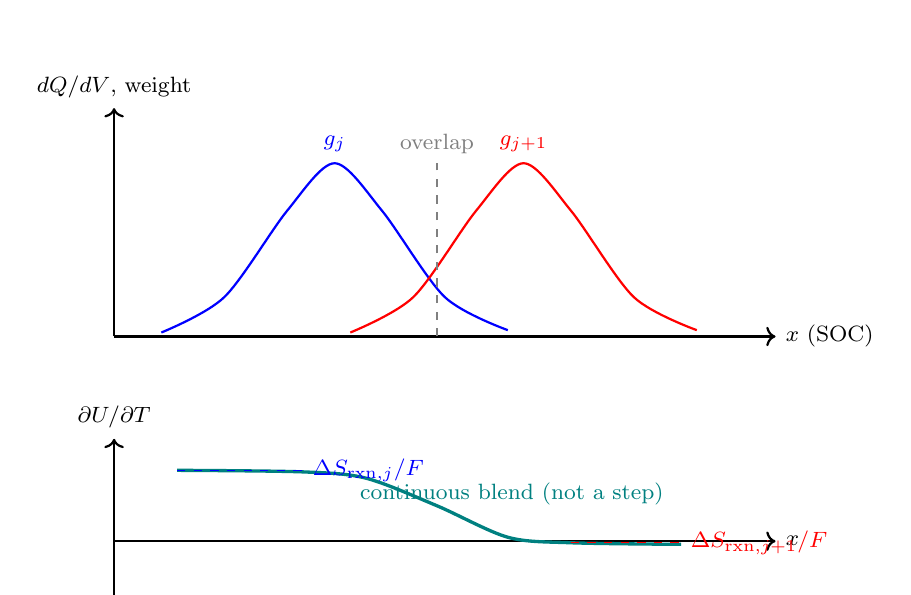
\begin{tikzpicture}[x=1.0cm,y=1.0cm]
  \draw[->,thick] (0,0) -- (8.4,0) node[right]{\footnotesize $x$ (SOC)};
  \draw[->,thick] (0,0) -- (0,2.9) node[above]{\footnotesize $dQ/dV$, weight};
  % two overlapping peaks g_j and g_{j+1}
  \draw[blue,thick,smooth] plot coordinates
    {(0.6,0.05)(1.4,0.5)(2.2,1.6)(2.8,2.2)(3.4,1.6)(4.2,0.5)(5.0,0.08)};
  \draw[red,thick,smooth] plot coordinates
    {(3.0,0.05)(3.8,0.5)(4.6,1.6)(5.2,2.2)(5.8,1.6)(6.6,0.5)(7.4,0.08)};
  \node[blue] at (2.8,2.45) {\footnotesize $g_j$};
  \node[red]  at (5.2,2.45) {\footnotesize $g_{j+1}$};
  % overlap region shading marker
  \draw[dashed,gray] (4.1,0)--(4.1,2.2);
  \node[gray,anchor=south] at (4.1,2.2) {\footnotesize overlap};
  % weighted average curve below: continuous slide between dS_j/F and dS_{j+1}/F
  \draw[->,thick] (0,-2.6) -- (8.4,-2.6) node[right]{\footnotesize $x$};
  \draw[->,thick] (0,-3.4) -- (0,-1.3) node[above]{\footnotesize $\partial U/\partial T$};
  \draw[teal,very thick,smooth] plot coordinates
    {(0.8,-1.7)(2.4,-1.72)(3.2,-1.8)(4.1,-2.15)(5.0,-2.55)(5.8,-2.62)(7.2,-2.64)};
  \draw[dashed,blue] (0.8,-1.7)--(2.4,-1.7) node[right,blue]{\footnotesize $\Delta S_{\mathrm{rxn},j}/F$};
  \draw[dashed,red]  (5.8,-2.62)--(7.2,-2.62) node[right,red]{\footnotesize $\Delta S_{\mathrm{rxn},j+1}/F$};
  \node[teal,anchor=west] at (3.0,-2.0) {\footnotesize continuous blend (not a step)};
\end{tikzpicture}
\caption{Peak overlap weighting. Top: two adjacent transition peaks $g_j,g_{j+1}$
($=$ the logistic occupation derivative, Eq.~\eqref{eq:logistic}) overlap in SOC. Bottom: the
observed entropy coefficient $\partial U/\partial T(x)$ slides \emph{continuously} from
$\Delta S_{\mathrm{rxn},j}/F$ to $\Delta S_{\mathrm{rxn},j+1}/F$, weighted by the local
$dQ/dV$ share $Q_jg_j/\sum_k Q_kg_k$ — a smooth blend, never a discontinuous step
(verified numerically, Table~\ref{tab:verify}).}
\label{fig:overlap}
\end{figure}

\subsection{완전식 — config 항까지 포함}
식~\eqref{eq:qrev_sum} 는 각 전이를 \emph{중심값}으로 본 ``단순식''이다. 봉우리 \emph{내부}의 config
$x$-의존(\S\ref{sec:config})까지 음함수 미분에 넣으면, 각 전이의 기여가
$\Delta S_{\rxn,j}/F + z_j\,R/F$($z_j\equiv(U_\oc(x)-U_j)/w_j$ = 중심에서 벗어난 정도)로 바뀌어
\begin{equation}
\frac{\partial U_\oc}{\partial T}(x)
   \;=\;\frac{\sum_j Q_j\,g_j\big(\Delta S_{\rxn,j}/F + z_j\,R/F\big)}{\sum_j Q_j\,g_j}
\label{eq:full}
\end{equation}
가 된다(``완전식''). 두 식의 차이가 곧 봉우리 내부 configurational 발산항이며, 측정급 비선형이 이
한 항에서 자동 생성된다.

\subsection{수치검증 — Chapter 1 코드로 round-trip}
위 두 식을 Chapter 1 의 실제 코드(\texttt{Anode\_Fit\_v11\_final.py}, \texttt{GRAPHITE\_STAGING\_LIT}
4 전이)로 검증했다. 방법: $T_1{=}292.15$, $T_2{=}298.15$\,K 두 온도에서 logistic 점유로 OCV 를 역산하고,
$\partial U_\oc/\partial T$ 를 유한차분(FD)으로 구해, $T_\mathrm{ref}{=}295.15$\,K 에서의 단순식
\eqref{eq:qrev_sum}$\cdot$완전식 \eqref{eq:full} 과 대조했다(전 $x\in[0.05,0.95]$, 181점).

\begin{table}[t]
\centering\small
\renewcommand{\arraystretch}{1.2}
\caption{유한차분(FD) vs.\ 단순식 \eqref{eq:qrev_sum}$\cdot$완전식 \eqref{eq:full} [mV/K]. 전이 파라미터
$\Delta S_{\rxn,j}=\{+29,0,-5,-16\}$ J\,mol$^{-1}$K$^{-1}$, $Q_j=\{0.10,0.12,0.25,0.50\}$. 발췌
5점 + 전체 175점(FD 부호교차 제외) 통계.}
\label{tab:verify}
\begin{tabular}{c c c c c c}
\toprule
$x$ & FD & 단순식 & 완전식 & $|$FD$-$단순$|$ & $|$FD$-$완전$|$ \\
\midrule
0.070 & $-0.3420$ & $-0.1455$ & $-0.3420$ & 0.1965 & $0.0000$ \\
0.200 & $-0.2318$ & $-0.1378$ & $-0.2318$ & 0.0940 & $0.0000$ \\
0.450 & $-0.1113$ & $-0.1124$ & $-0.1113$ & 0.0011 & $0.0000$ \\
0.700 & $+0.0115$ & $-0.0667$ & $+0.0115$ & 0.0782 & $0.0000$ \\
0.930 & $+0.2790$ & $+0.1543$ & $+0.2790$ & 0.1247 & $0.0000$ \\
\midrule
\multicolumn{4}{l}{\footnotesize 전체 175점 max abs err} & 0.1841 & $0.000000$ \\
\multicolumn{4}{l}{\footnotesize 전체 175점 mean abs err} & 0.0742 & $0.000000$ \\
\bottomrule
\end{tabular}
\end{table}

결과(표~\ref{tab:verify}): \textbf{완전식 \eqref{eq:full} 은 FD 와 부동소수점 정밀도 수준에서 완벽
일치}(max abs err $=0$ mV/K). 단순식 \eqref{eq:qrev_sum} 은 체계적 오차 최대 $0.18$ mV/K 를 남기는데,
이는 결함이 아니라 \emph{의도적으로 분리한 config 항}의 크기다 — 완전식 $-$ 단순식이 정확히 봉우리 내부
configurational 발산항($\sum_j Q_jg_j z_j R/F$, 전 범위 $[-0.21,+0.14]$ mV/K)이다. 또한 인접 전이 경계
4곳 모두에서 FD 가 두 전이의 $\Delta S/F$ 사이 값을 연속으로 취해(예: $j{=}0\!-\!1$ 중간 $x{=}0.815$ 에서
$+0.10$ mV/K $\in[0,+0.30]$), \emph{계단이 아닌 연속 블렌드}임이 확인됐다(전이 경계 최대 변화율
$\le13$ µV/K/step).

\begin{keybox}
\textbf{측정급 비선형이 모델 내에서 자동 생성된다.} 임시 계단 함수나 외부 입력 없이, logistic 점유
\emph{분포 자체}에서 (i) 봉우리 겹침 가중과 (ii) 봉우리 내부 config 발산 두 출처가 측정급 비선형
$\partial U/\partial T(x)$(최대 $\pm0.21$ mV/K 변동)를 만든다. 곧 $\Delta S_{\rxn,j}$ 를 ``전이당 상수''
로 두고 분포가 나머지를 채우게 하면 충분하다 — $\Delta S_{\rxn,j}(x)$ 를 임의 함수로 둘 필요가 없다
(\S\ref{sec:limits} 에서 근사 타당성 판정).
\end{keybox}

% ====================================================================
\section{상호작용과 히스테리시스 — 분포의 변형과 분기}\label{sec:omega}
% ====================================================================
지금까지의 분포는 상호작용 없는 이상 격자기체였다($\Omega=0$). 실제 흑연 stage 에는 평균장 상호작용
$\Omega$ 가 있어 봉우리를 좁히고, 충방전 경로가 갈리는 히스테리시스가 있다. 두 효과를 분포 관점에서
닫는다.

\subsection{유효 폭 $w_\eff(\Omega)$ — 상호작용이 봉우리를 좁힌다}
식~\eqref{eq:mu_bw} 의 정규용액 격자기체에서 평형 등온선 기울기는
\begin{equation}
\frac{\dd V_\eq}{\dd\xi}
   \;=\;\frac{RT}{F}\Big[\frac{1}{\xi(1-\xi)}\;-\;\frac{2\Omega}{RT}\Big]
\label{eq:isotherm_slope}
\end{equation}
이다(상호작용 항 $\Omega(1-2\xi)$ 의 미분 $-2\Omega$ 가 더해짐). 중심 $\xi=\tfrac12$ 에서 기울기는
$(4RT-2\Omega)/F$ 로, $\Omega>0$ 이 봉우리를 \emph{좁힌다}(같은 $x$ 폭에 더 가파른 logistic). 이상
격자기체($\Omega=0$)의 중심 기울기 $4RT/F=4w F\cdot\!(1/F)$ 와 정합시키면 \emph{유효 폭}
\begin{equation}
\boxed{\;w_\eff\;=\;\frac{w}{\,1-\Omega/(2RT)\,}\;}\qquad(\Omega<2RT)
\label{eq:weff}
\end{equation}
이 정의된다. $\Omega\to0$ 에서 $w_\eff\to w=RT/F$ 로 환원되고, $\Omega\to2RT^-$ 에서
$w_\eff\to\infty$ 로 발산 — 이것이 \emph{상분리 임계}다(분포가 둘로 쪼개져 bimodal, 봉우리가 무한히
좁아진 plateau).

\begin{figure}[t]
\centering
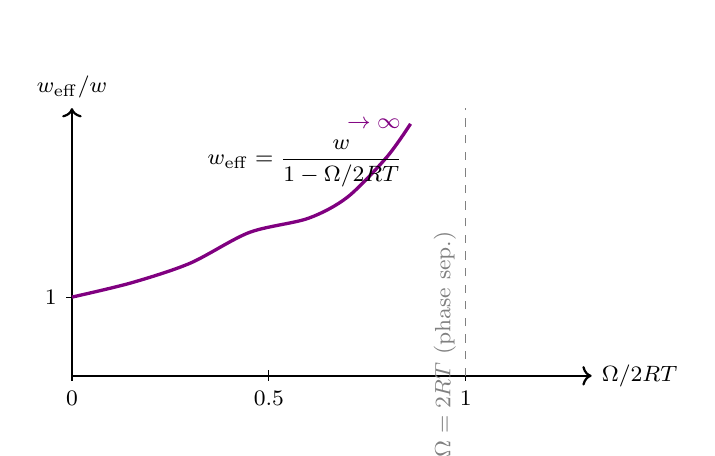
\begin{tikzpicture}[x=1.0cm,y=1.0cm]
  \draw[->,thick] (0,0) -- (6.6,0) node[right]{\footnotesize $\Omega/2RT$};
  \draw[->,thick] (0,0) -- (0,3.4) node[above]{\footnotesize $w_\mathrm{eff}/w$};
  \foreach \t/\lab in {0/0,2.5/0.5,5/1}{\draw (\t,0.07)--(\t,-0.07) node[below]{\footnotesize \lab};}
  \draw (0.07,1)--(-0.07,1) node[left]{\footnotesize $1$};
  % w_eff/w = 1/(1 - u), u = Omega/2RT, x = 5u
  \draw[violet,very thick,smooth] plot coordinates
    {(0,1.0)(0.75,1.18)(1.5,1.43)(2.25,1.82)(3.0,2.0)(3.5,2.27)(4.0,2.78)(4.3,3.2)};
  \draw[dashed,gray] (5,0)--(5,3.4);
  \node[gray,anchor=south,rotate=90] at (5,0.4) {\footnotesize $\Omega=2RT$ (phase sep.)};
  \node[violet,anchor=east] at (4.3,3.2) {\footnotesize $\to\infty$};
  \node[anchor=west] at (1.6,2.7) {\footnotesize $w_\mathrm{eff}=\dfrac{w}{1-\Omega/2RT}$};
\end{tikzpicture}
\caption{Interaction narrows the occupation distribution. The effective logistic width
$w_\mathrm{eff}=w/(1-\Omega/2RT)$ diverges as the mean-field repulsion approaches the
phase-separation threshold $\Omega\to2RT^-$, where the distribution splits into a bimodal
(two-phase) form and the entropy coefficient flattens into a plateau. For $\Omega=0$ the ideal
lattice gas recovers $w=RT/F$.}
\label{fig:weff}
\end{figure}

\textbf{config 부분몰 엔트로피 모양도 변형된다.} 좁아진 봉우리에서는 같은 $x$ 폭에 $\ln[\xi/(1-\xi)]$ 가
더 가파르게 쓸리므로(식~\eqref{eq:dVdT} 둘째 항), 봉우리 내부 $\partial U/\partial T$ 변동이
\emph{증폭}된다. $\Omega\to2RT$ 에서 발산해 상분리 plateau 가 되면, 그 구간의 엔트로피 계수는
\emph{평탄}해지고 경계에서 불연속이 된다(2상 공존서 부분몰 엔트로피 일정). 곧 $w\to w_\eff(\Omega)$
치환만으로 상호작용이 측정 계수에 들어간다.

\begin{warnbox}
$\Omega$ 자체가 약한 온도 의존을 가지면 $\partial w_\eff/\partial T$ 가 $\partial U/\partial T$ 에 2차
기여를 한다 — 본 장에서는 소수 항으로 명시만 하고, 주 효과는 폭 치환 \eqref{eq:weff} 로 본다.
\end{warnbox}

\subsection{히스테리시스 — 충/방전 분기별 엔트로피 계수}
흑연 OCV 는 충방전 사이 history-dependent(준안정 stacking, stage II 무질서)라 단일 $\partial U/\partial T$
가 경로의존이다 \cite{hysteresis2018}. 분기 $d$(충전/방전)의 전이 중심은
$U_j^{(d)}=U_j\pm\tfrac12\Delta U_j^\mathrm{hys}$ 로 갈리고, 각 분기의 엔트로피 계수는 식~\eqref{eq:qrev_sum}
를 분기 봉우리 $g_j^{(d)}$ 로 평가한
\begin{equation}
\frac{\partial U_\oc^{(d)}}{\partial T}
   \;=\;\frac{1}{F}\,\frac{\sum_j Q_j\,g_j^{(d)}\,\Delta S_{\rxn,j}}{\sum_j Q_j\,g_j^{(d)}}
\label{eq:hys_branch}
\end{equation}
이다. \textbf{가역 발열에 들어가는 것은 두 분기의 평균}이다:
\begin{equation}
\boxed{\;\frac{\partial U^\mathrm{rev}}{\partial T}
   \;=\;\tfrac12\Big(\frac{\partial U^\mathrm{ch}}{\partial T}+\frac{\partial U^\mathrm{dis}}{\partial T}\Big)\;}
\label{eq:hys_rev}
\end{equation}
— 이것이 가역 발열~\eqref{eq:qrev} 의 열역학적 $\Delta S$ 다. 한편 히스 gap $\Delta U^\mathrm{hys}$
\emph{자체}는 entropy production(비가역열 $\propto I\,\Delta U^\mathrm{hys}$)이라 $\partial/\partial T$
와 분리해 계산한다.

\begin{warnbox}
\textbf{가역과 비가역의 경계(혼동 금지).} 가역 발열은 \emph{평균 분기}~\eqref{eq:hys_rev} 의 엔트로피
계수로 정의하고, 히스 gap 이 만드는 entropy production $\sigma\ge0$ 은 비가역열로 분리한다. 둘을
한 $\partial U/\partial T$ 에 섞으면 안 된다. 경로의존 측정 불확실도의 정량은 본 장 범위 밖이다(공백).
\end{warnbox}

% ====================================================================
\section{극한과 코너 — ``$\Delta S_{\rxn,j}$ 상수'' 근사의 타당성}\label{sec:limits}
% ====================================================================
세운 식들이 알려진 극한에서 옳게 거동하는지 검산하고, 그로부터 ``$\Delta S_{\rxn,j}$ 를 전이당 상수로
둔다''는 모델링 선택이 언제 타당한지 판정한다.

\begin{table}[t]
\centering\small
\renewcommand{\arraystretch}{1.25}
\caption{극한 코너 검산. $\xi$ = 탈리튬화 진행률(\S\ref{sub:sign}). config = 식~\eqref{eq:dVdT} 둘째 항.}
\label{tab:limits}
\begin{tabular}{l l l}
\toprule
극한 & $\partial U/\partial T$ 거동 & 물리/검증 \\
\midrule
$\xi\to1$ (희박 Li) & config $\to+\infty$ & 저-$x$ 큰 양 $\Delta S$($+29$)의 주원천 \\
$\xi\to0$ (만충) & config $\to-\infty$ & 만충 정렬, 부분몰 엔트로피 음 발산 \\
$\xi=\tfrac12$ (중심) & $=\Delta S_{\rxn,j}/F$ & config $=0$, 표준값 회수 \\
$\Omega\to2RT^-$ & $w_\eff\to\infty$, plateau & 상분리 임계(평탄$\cdot$불연속) \\
단일 봉우리(겹침 0) & $=\Delta S_{\rxn,j}/F+$config & 가중식 \eqref{eq:qrev_sum} 이 단일 전이로 환원 \\
고온 & electronic $\propto T$ 우세화 & FD Sommerfeld \eqref{eq:Sel} \\
\bottomrule
\end{tabular}
\end{table}

표~\ref{tab:limits} 의 여섯 코너가 모두 물리적으로 옳다 — 단일 봉우리 한계에서 가중식~\eqref{eq:qrev_sum}
이 한 전이의 $\Delta S_{\rxn,j}/F$ 에 config 를 더한 형태로 정확히 환원되고, 중심에서 표준값을 회수하며,
$\Omega$ 임계에서 상분리 plateau 를 낳는다.

\begin{keybox}
\textbf{근사 타당성 판정.} ``$\Delta S_{\rxn,j}$ 를 전이당 상수''로 두는 근사는, 중심 표준값
(vib+electronic 중심 포함)이 \emph{전이 폭 안에서 천천히 변할 때} 타당하다. 봉우리 내부의 \emph{급변}은
config 분포항이 담으므로(상수로 둘 수 없는 게 아니라, 상수로 두고 분포가 채운다), 측정 $\partial U/\partial
T(x)$ 의 비선형은 (i) 봉우리 겹침 가중 + (ii) 봉우리 내부 config 두 출처로 \emph{자동 생성}된다 —
$\Delta S_{\rxn,j}(x)$ 를 임의 함수로 둘 필요가 없다. \emph{예외}: vib/electronic 이 한 전이 폭 안에서
급변하면(LCO MIT 게이트가 한 전이 안에서 켜지는 경우) 그 항만 $x$-의존을 유지한다(\S\ref{sec:vibel}).
\end{keybox}

% ====================================================================
\section{합성 — 가역 발열 프로파일과 한계}\label{sec:synth}
% ====================================================================
이제 분포에서 세운 엔트로피 계수가 실제 흑연 곡선$\cdot$가역 발열로 어떻게 닫히는지 종합한다.

\subsection{흑연 staging 엔트로피 프로파일 — 분포 부호와 문헌의 일치}
세 분포가 예측하는 부호가 흑연의 측정 엔트로피 프로파일과 정합한다. 저-$x$(희박, $\xi\to1$)에서 config
부분몰이 $+$ 로 크게 발산 → $\Delta S>0$; 고-$x$(만충)에서 vib baseline 이 음으로 → $\Delta S<0$.
문헌이 정확히 이 부호 교대를 보고한다: 저 Li 분율($x<0.2$--$0.25$)에서 $\Delta S>0$
(configurational), 고 분율에서 $\Delta S<0$(vibrational) — Reynier, Yazami, Fultz \cite{reynier2003};
Allart 등 \cite{allart2018} 정량 $\Delta S\approx+29$ J\,mol$^{-1}$K$^{-1}$@$x{=}0.08$
(전극 분리 기준, $\Delta S/F\approx+0.3$ mV/K), $-5\sim-16$@$x>0.5$; MCMB 흑연
$\partial U/\partial T\approx+3\sim4$ mV/K @저-$x$, $\sim0.2$ SOC 부근 부호 반전 \cite{msmr_partII}
(보고 척도가 더 큰 것은 측정$\cdot$기준 정의 차이 — 부호 교대 추세가 본 장 분포 예측과 일치하는 것이
요지). stage\,$2\!\to\!1$($x\approx0.5$)의 엔트로피 재증가(이상 거동)도 보고된다
\cite{reynier2003,allart2018}.

\begin{srcbox}
★\textbf{Chapter 1 정합(정량).} Chapter 1 \texttt{GRAPHITE\_STAGING\_LIT} 의 전이별 $\Delta S_{\rxn,j}$ 는
$+29\to0\to-5\to-16$ J\,mol$^{-1}$K$^{-1}$(stage $4\!\to\!3\!\to\!2\mathrm L\!\to\!2\!\to\!1$)로, 문헌 흑연
$\Delta S(x)$ \cite{allart2018} 와 \emph{부호$\cdot$규모가 정량 일치}한다($+29$@저-$x$, $-16$@$x>0.5$ 정확
대응; 표~\ref{tab:ds}). 곧 \S\ref{sec:config}--\S\ref{sec:vibel} 의 분포가 준 부호가 임의값이 아니라
측정에 닿아 있음을 뒷받침한다.
\end{srcbox}

\begin{table}[t]
\centering\small
\renewcommand{\arraystretch}{1.2}
\caption{Chapter 1 전이별 $\Delta S_{\rxn,j}$(=중심 표준값 $\Delta S^0_j$) ↔ 문헌 흑연 $\Delta S(x)$
(Allart 등 \cite{allart2018}, 전극 분리).}
\label{tab:ds}
\begin{tabular}{l c c c}
\toprule
전이 & $x$ 범위 & Ch1 $\Delta S_{\rxn,j}$ [J\,mol$^{-1}$K$^{-1}$] & 문헌 $\Delta S(x)$ \\
\midrule
$4\!\to\!3$ & 0.08–0.16 & $+29.0$ & $+29$ @\,$x{=}0.08$ (양 끝, 정확) \\
$3\!\to\!2\mathrm L$ & 0.16–0.25 & $0.0$ & 중간 하강 구간 $0\!\to\!-16$ (범위) \\
$2\mathrm L\!\to\!2$ & 0.25–0.50 & $-5.0$ & 중간 하강 구간 (범위) \\
$2\!\to\!1$ & 0.50–1.00 & $-16.0$ & $-16$ @\,$x{>}0.5$ (양 끝, 정확) \\
\bottomrule
\end{tabular}

\smallskip
{\footnotesize $\dagger$ Chapter 1 의 4 주요 plateau 전이와 Allart 등 \cite{allart2018} 의 세분 region(dilute
LiC$_{24}$ 포함, 양 끝 reg IV/reg I)은 $x$-경계가 $1{:}1$ 이 아니다. \emph{양 끝}($+29$ @저-$x$, $-16$ @$x{>}0.5$)
은 정확 대응하고, 중간 두 전이는 $\Delta S$ 가 $0\to-16$ 으로 하강하는 \emph{구간 안}에 놓인다(점-대-점이 아닌
범위 정합). 해상도 차이일 뿐 추세$\cdot$부호는 일관.}
\end{table}

엔탈피 쪽은 \emph{기준 차이}에 주의한다. Chapter 1 의 $\Delta H_{\rxn,j}$ 는 \emph{전이별}(differential)
반응 엔탈피이고, calorimetry 의 형성 엔탈피(LiC$_6$ $-13.9$, LiC$_{12}$ $-24.8$ kJ/mol\,Li
\cite{chemmater2015})는 \emph{누적}(formation, graphite+Li 금속 기준)이라 직접 등치할 수 없다 — 비교하려면
형성 엔탈피의 $x$-미분으로 환산해야 한다. Chapter 1 내부에서는 $\Delta H_{\rxn,j}$ 가
$U_j\cdot\Delta S_{\rxn,j}$ 와 식~\eqref{eq:coeff} 의 역관계로 일관된다(예: stage\,$2\!\to\!1$ 에서
$-FU+FT\,\partial U/\partial T=-13.0$ kJ/mol, 표값과 일치). 부호$\cdot$규모는 분포가 주는 항들과 무모순이다.

\subsection{다온도 $dQ/dV$ 에서 $\partial U/\partial T$ 를 뽑는 경로}\label{sub:estimate}
실데이터에서 전이별 $\Delta S_{\rxn,j}$ 를 얻는 길은, 여러 온도 $T_k$ 의 $dQ/dV$ 를 Chapter 1 모델로
동시에 맞춰 전이별 중심 $U_j(T_k)$ 의 온도 기울기 $\partial U_j/\partial T$ 를 읽는 것이다. 방법론적
template 은 다중 반응 모델의 $OCV(T)$ 회귀다:
\begin{itemize}[leftmargin=1.4em,itemsep=2pt]
\item \textbf{MSMR(Multi-Species, Multi-Reaction)} 은 흑연 OCV 를 반응별 항의 합으로 보고, 각 반응의
$U_j^0(T)$ 를 온도의 연속함수(저차 다항)로 두어 엔트로피 계수를 추정한다 \cite{msmr_partI,msmr_partII}.
이는 Chapter 1 의 전이별 logistic 구조(=격자기체 점유 분포)와 직접 대응한다(반응 $j\leftrightarrow$
전이 $j$).
\item \textbf{Potentiometric/dynamic 엔트로피 측정} 은 $OCV(T)$ 온도 응답을 직접 재며, 표준 protocol 과
불확도(full-cell $\partial U/\partial T$ 0.3--0.5 mV/K @0--20\% SOC, std.dev $\sim$µV/K)가 보고된다
\cite{standardised2024}.
\item \textbf{$dQ/dV$ 기반 부분몰 엔트로피} prototype: incremental capacity 와 entropy profiling 을 결합해
격자기체(Bragg--Williams 확장) 틀에서 부분몰 $\Delta S\cdot\Delta H$ 를 얻은 선례 \cite{occupation2019}
(dilute $0<x<0.1$ 한정; 본 장은 원문 식 미확보로 \emph{방법 수준}만 인용).
\end{itemize}

\begin{keybox}
\textbf{본 장의 각.} 위 선례는 대부분 $OCV(T)$ 또는 dilute 한계를 쓴다. 본 장은 \emph{전} 전이의
점유 \emph{분포}를 명시 전개해, 측정 $\partial U/\partial T(x)$ 의 비선형이 봉우리 겹침 + 봉우리 내부
config 에서 \emph{자동 생성}됨을 수치로 닫았다(\S\ref{sec:overlap}). MSMR 을 template, Allart 값을
검증, Bernardi 를 출구로 삼는 이 경로의 정확도 실증은 실데이터 round-trip(후속 단계)이다.
\end{keybox}

\textbf{피팅 함정(문헌 경고).} 저율 준평형 데이터 사용(고율은 동역학 오염), 평활은 가장 좁은 peak
반높이 폭의 $1/5$ 이하(과평활→폭 양의 편향), peak 분해 시 전이 중심 우선, 연속함수$\cdot$저차로 과적합
억제 \cite{msmr_partI,msmr_partII}. Chapter 1 의 $R_n\cdot$동역학 꼬리는 \emph{비가역} 성분이므로,
$\partial U/\partial T$ 추정 전에 분극$\cdot$히스를 분리해야 한다($V_n=V_\mathrm{app}-\sigma_d|I|R_n$).

\subsection{가역 발열 프로파일}
전이별 $\Delta S_{\rxn,j}$ 와 분포항이 정해지면 가역 발열은 식~\eqref{eq:qrev}$\cdot$\eqref{eq:qrev_sum}
로 닫힌다 — SOC 에 따라 $\Delta S(x)$ 부호가 바뀌어(저-$x$ 양 $\Rightarrow$ 방전서 $\dot Q_\rev>0$ 발열,
고-$x$ 음 $\Rightarrow$ 흡열) 흡$\cdot$발열이 교대한다. stage\,$2\!\to\!1$($x\approx0.5$)의 큰 음의
$\Delta S$ 는 가역 발열의 두드러진 신호를 남긴다. 이는 calorimetry 의 가역 흡열 직접 관측과 정합한다
\cite{standardised2024}. \textbf{분포 관점의 요지}: 이 흡$\cdot$발열 교대는 ``리튬(+전자+포논) 점유
분포를 한 SOC 에서 다른 SOC 로 재배열할 때 흩어짐이 늘거나(흡열) 주는(발열)'' 직접 결과다.

\textbf{한계$\cdot$갭(정직).} (1) $dQ/dV(T)$ 직접 추정의 정확도는 실데이터 round-trip 으로만 확정(후속).
(2) 히스 하 경로의존 $\partial U/\partial T$ 불확실도 정량 미확보. (3) Electrochim.\,Acta 2019 prototype
의 모델 식$\cdot$절대 $\Delta S/\Delta H$ 원문 미확보(유료) — 방법만 인용. (4) DFT 절대 엔탈피는
interlayer 기술 난점으로 실험 우선 \cite{jpcc2021}. (5) 형성↔전이별 엔탈피 환산식은 본 장 범위 밖.
(6) Bragg--Williams 평균장은 단거리 상관$\cdot$stage 초격자를 평균화 — 정량 stage 경계는 근사.

% ====================================================================
\section*{맺음 — 다음 단계}
\addcontentsline{toc}{section}{맺음}
% ====================================================================
본 장은 흑연 코인 하프셀의 엔트로피 계수$\cdot$가역 발열을 \emph{점유 분포의 통계열역학}으로 세웠다.
골격은 한 줄이었다 — 격자기체 분배함수 $Z_1=1+e^{-\beta\Delta\mu}$ 에서 점유 분포 $\avg{n}$ 를 얻고
(그것이 곧 Chapter 1 의 logistic 이고 폭 $w=RT/F$ 가 분포의 흩어짐), 그 분포의 흩어짐에서
configurational 엔트로피 $S_\config=-R\sum p\ln p$ 와 부분몰 $-R\ln[\theta/(1-\theta)]$ 를 끌어내고
(이것이 봉우리 내부 $x$-의존, 이미 $w$ 가 담음 — 이중계산 B 금지), 격자 진동(포논 BE)과 전도 전자
(FD/Sommerfeld) 두 분포를 더해 총 엔트로피 계수 \eqref{eq:master} 를 세웠다. 그 위에서 봉우리 겹침
가중 \eqref{eq:qrev_sum} 을 음함수 미분으로 닫고 Chapter 1 코드로 부동소수점 수준까지 수치검증했으며
(표~\ref{tab:verify}), 상호작용 $w_\eff(\Omega)$$\cdot$히스 분기$\cdot$극한 코너를 봉합하고, Bernardi
가역열을 ``분포 재배열 열''로 다시 읽었다.

핵심 결론: \textbf{측정 $\partial U/\partial T(x)$ 의 비선형은 임의 함수가 아니라 점유 분포에서 자동
생성된다} — 봉우리 겹침과 봉우리 내부 config 두 출처가 측정급 변동을 만들고, $\Delta S_{\rxn,j}$ 는
전이당 상수로 충분하다. \textbf{다음}: (i) 실데이터 다온도 $dQ/dV$ round-trip 으로 추정 정확도 실증,
(ii) LCO 하프셀 MIT 게이트의 $\Delta S_e^{\,\mathrm{gate}}$ 정량(Chapter 1 v9 전자항), (iii) Chapter 1
과의 v9 통합(가역/비가역 발열을 한 인과 사슬로). 교수님 검토 입력 대기.

% ====================================================================
\begin{thebibliography}{99}
\bibitem{bernardi1985} D. Bernardi, E. Pawlikowski, J. Newman, ``A General Energy Balance for Battery Systems,'' \emph{J. Electrochem. Soc.} \textbf{132}(1), 5--12 (1985). DOI: 10.1149/1.2113792.
\bibitem{newman} J. Newman, K. E. Thomas-Alyea, \emph{Electrochemical Systems}, 3rd ed., Wiley (2004). (OCV($T$): slope $=\Delta S$, intercept $=\Delta H$.)
\bibitem{reynier2003} Y. Reynier, R. Yazami, B. Fultz, ``The entropy and enthalpy of lithium intercalation into graphite,'' \emph{J. Power Sources} \textbf{119--121}, 850--855 (2003). DOI: 10.1016/S0378-7753(03)00285-4.
\bibitem{allart2018} D. Allart \emph{et al.}, ``Model of Lithium Intercalation into Graphite by Potentiometric Analysis with Equilibrium and Entropy Change Curves of the Graphite Electrode,'' \emph{J. Electrochem. Soc.} \textbf{165}(2), A380 (2018). DOI: 10.1149/2.1251802jes.
\bibitem{occupation2019} ``Transitions of lithium occupation in graphite: A physically informed model in the dilute lithium occupation limit supported by electrochemical and thermodynamic measurements,'' \emph{Electrochimica Acta} (2019). DOI: 10.1016/j.electacta.2019.135634. [방법 수준 인용 — 원문 식 미확보.]
\bibitem{chemmater2015} ``Intercalation Compounds from LiH and Graphite: Relative Stability of Metastable Stages\ldots,'' \emph{Chem. Mater.} \textbf{27} (2015). DOI: 10.1021/acs.chemmater.5b00235. [형성 ΔH calorimetry — abstract tier.]
\bibitem{jpcc2021} ``Thermodynamic Analysis of Li-Intercalated Graphite by First-Principles with Vibrational and Configurational Contributions,'' \emph{J. Phys. Chem. C} \textbf{125} (2021). DOI: 10.1021/acs.jpcc.1c08992. [abstract tier.]
\bibitem{msmr_partI} ``Quantifying the Entropy and Enthalpy of Insertion Materials for Battery Applications Via the Multi-Species, Multi-Reaction Model,'' \emph{J. Electrochem. Soc.} (2024). DOI: 10.1149/1945-7111/ad1d27.
\bibitem{msmr_partII} ``Quantifying the Temperature Dependence of the MSMR Model Part II: Estimation of Entropy Coefficient for Meso-Carbon Micro-Bead Graphite,'' \emph{J. Electrochem. Soc.} (2024). DOI: 10.1149/1945-7111/ad70d9.
\bibitem{standardised2024} ``A Standardised Potentiometric Method for the Effective Parameterisation of Reversible Heating in a Lithium-Ion Cell,'' \emph{J. Electrochem. Soc.} (2024). DOI: 10.1149/1945-7111/ad4918.
\bibitem{hysteresis2018} ``Uncertainties in entropy due to temperature path dependent voltage hysteresis in Li-ion cells,'' \emph{J. Power Sources} (2018). DOI: 10.1016/j.jpowsour.2018.05.060.
\bibitem{hill} T. L. Hill, \emph{An Introduction to Statistical Thermodynamics}, Addison-Wesley (1960); Dover reprint (1986). (Grand canonical 분배함수, 격자기체 점유 $\avg{n}$, lattice-gas $\leftrightarrow$ Ising 대응.)
\bibitem{bazant2013} M. Z. Bazant, ``Theory of Chemical Kinetics and Charge Transfer Based on Nonequilibrium Thermodynamics,'' \emph{Acc. Chem. Res.} \textbf{46}(5), 1144--1160 (2013). DOI: 10.1021/ar300145c. (정규용액 격자기체 OCV $\mu(\theta)=RT\ln[\theta/(1-\theta)]+\Omega(1-2\theta)$, 상분리 임계 $\Omega>2RT$.)
\bibitem{ashcroftmermin} N. W. Ashcroft, N. D. Mermin, \emph{Solid State Physics}, Holt--Saunders (1976), Ch.~2. (전자 비열$\cdot$엔트로피 Sommerfeld 전개 $S_\elec=\tfrac{\pi^2}{3}\kB^2 T\,g(E_F)$.)
\bibitem{huggins2009} R. A. Huggins, \emph{Advanced Batteries: Materials Science Aspects}, Springer (2009). (삽입 전극 평형 전위와 부분몰 열역학량의 관계 — 교과서 tier.)
\end{thebibliography}

\end{document}
